\section{Evaluation}\label{sec:eval}

We evaluate the procedure through two research questions.

\begin{enumerate}[start=1,label={\bfseries RQ\arabic*:}, itemindent=2em, ref=\bfseries RQ\arabic*, itemsep=0.1em]
\item \label{rq:structural} Which parameters of the input formula drive the cost of the search, and
how does it scale in each?
\item \label{rq:practicality} Is the procedure practical on the flat, one-level TCTL queries
engineers write for \textsc{Uppaal}?
\end{enumerate}

\noindent
\ref{rq:structural} asks where the \textsc{ExpTime} bound of Theorem~\ref{thm:alg} is felt and where
it is not; \ref{rq:practicality} asks the complementary question, whether the queries a specification
is actually checked against lie in the expensive regime.

\paragraph{Benchmark and method.}
No standard suite exists for TCTL \emph{satisfiability}, and there is no second implementation to
compare against, so the study characterises one procedure rather than ranking two. We generate $333$
parameterised instances. For \ref{rq:structural} each family varies a single term of
$2^{O(n)}\cdot M^{O(n^{2})}$ with the others fixed: the number of \emph{simultaneously live}
formula-clocks $k$, obtained by conjoining $k$ independent timed untils; the \emph{nesting depth} $d$
of a timed double-check; the largest constant $M$, swept by powers of two to $2^{20}$; and the
propositional \emph{size} $m$. Each ships matched satisfiable and unsatisfiable variants, so witness
cost and refutation cost are separated. For \ref{rq:practicality} we generate the canonical
\textsc{Uppaal} shapes over atomic propositions, each swept along payload size $m\le1024$ and time
bound $b\le2^{20}$.

We report the number of tableau \emph{nodes} as the primary measure. It is a deterministic function
of the formula, independent of the machine, and it is what Lemma~\ref{lem:finiteness} bounds; every
growth law below is fitted to it. Wall-clock time and peak resident memory are reported as maxima
only. Each instance was given $600$\,s and a $10$\,GB resident-memory cap, run serially on an
Apple~M4~Pro; timing is the median of three runs for instances under $5$\,s and a single run above.
\textbf{No instance timed out, and none reached the memory cap.}

\begin{table}[t]\centering
\caption{\textbf{\ref{rq:structural}: cost drivers.} One row per family and verdict, over the whole sweep.
The growth law is fitted to the \emph{node count}, which is a deterministic function of the formula;
wall-clock is reported as a maximum only, since instrumentation floors it at $0.2$\,s. No instance
timed out or reached the memory cap.}\label{tab:rq1}
\small\setlength{\tabcolsep}{5pt}
\begin{tabular}{llccrrrr}
\toprule
Factor & Verdict & Range & Nodes & $R^2$ & max nodes & max $t$\,(s) & max mem\,(MB)\\
\midrule
Clocks $k$ & SAT & 1--20 & $\mathbf{1.93^{k}}$ & 1.00 & 4{,}194{,}836 & 494.57 & 3628 \\
Clocks $k$ & UNSAT & 1--20 & linear & 0.99 & 279 & 0.20 & 2 \\
Depth $d$ & UNSAT & 1--12 & $d^{2.48}$ & 1.00 & 211{,}527 & 11.16 & 178 \\
Depth $d$ & SAT & 1--12 & $d^{1.84}$ & 0.98 & 10{,}283 & 0.49 & 9 \\
Size $m$ & SAT & 1--1024 & $m^{0.63}$ & 0.94 & 1{,}038 & 0.82 & 32 \\
Const $M$ & SAT & 2--1048576 & flat & --- & 286 & 0.20 & 4 \\
Const $M$ & UNSAT & 1--1048576 & flat & --- & 401 & 0.20 & 2 \\
\bottomrule
\end{tabular}
\end{table}


\paragraph{\ref{rq:structural}: one exponential driver, and it is not nesting.}
Table~\ref{tab:rq1} ranks the four factors, and they separate sharply.

\emph{Clock simultaneity is the only exponential axis.} On satisfiable instances the node count is
$1.93^{k}$ with $R^{2}=1.00$ over the whole sweep $k=1..20$, a clean doubling per added clock, ending
at $4.19$M nodes, $3.6$\,GB and $495$\,s. This is the $M^{O(n^{2})}$ handle: $k$ clocks live at once
means a DBM of dimension $k+1$, and a witness has to meet all $k$ windows together, so the search
enumerates their product.

\emph{Nesting depth is polynomial.} Refutation grows as $d^{2.48}$ ($R^{2}=1.00$) and a witness as
$d^{1.84}$, so depth~$12$ costs $211$k nodes and $11$\,s unsatisfiable, $10$k nodes and half a second
satisfiable. Nesting is an order of magnitude cheaper than the bound permits, because the memoised
graph collapses the repeated structure of the nested check instead of unfolding it.

\emph{Neither $M$ nor formula size is a driver.} The node count is constant at $293$ across six
orders of magnitude of $M$, from $1$ to $2^{20}$: a zone represents a large bound symbolically, and
$\cong_M$ leaves the realised set identical. Propositional size is sublinear, $m^{0.63}$, so a
payload of $1024$ atoms realises $1038$ nodes. The closure grows; the search does not.

\emph{The witness/refutation asymmetry runs in both directions,} and which way depends on what the
formula demands. On clocks the satisfiable side is the expensive one, $4.19$M nodes against $279$: a
model must meet every obligation at once, whereas a single contradiction closes the refutation
outright. On depth the order reverses, $211$k against $10$k: the witness is short-circuited at the
first accepting branch, while the refutation has to exhaust the graph. The ranking is therefore
$\textit{clocks}\gg\textit{depth}\gg\{M,\textit{size}\}$, with the exponential confined to
satisfiable instances of the first.

\begin{figure}[t]\centering
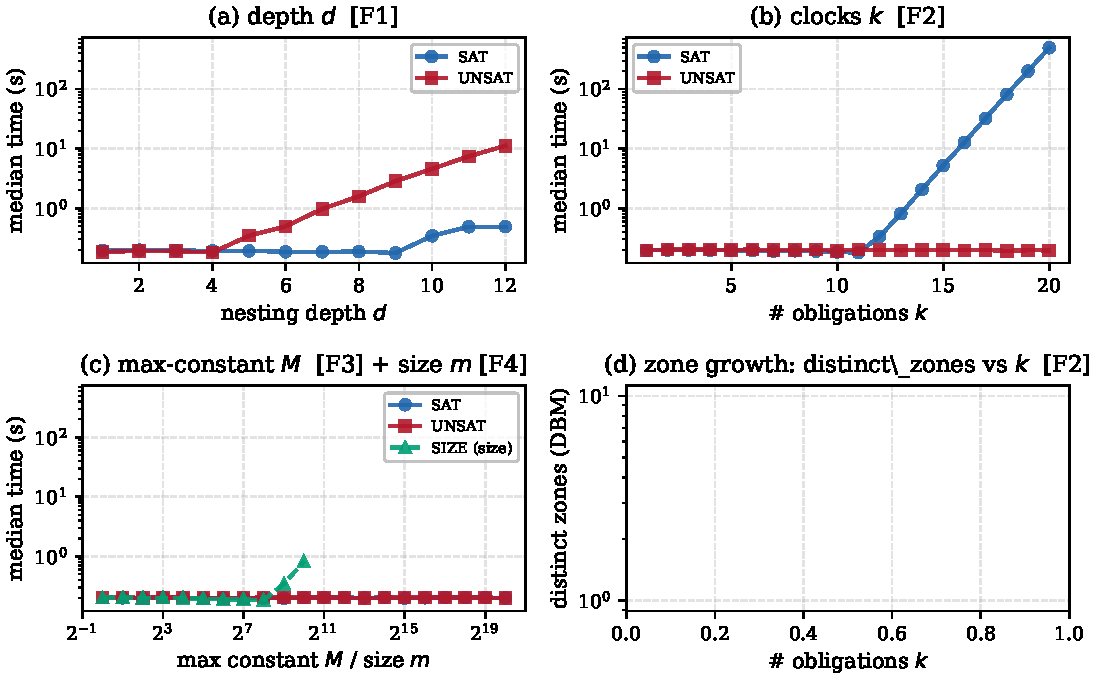
\includegraphics[width=0.72\textwidth]{figs/fig_drivers.pdf}
\caption{\ref{rq:structural} cost drivers: median runtime against each parameter, satisfiable and
unsatisfiable shown separately. Clock simultaneity is exponential, depth is polynomial, and the
constant $M$ and the propositional size are flat.}\label{fig:drivers}
\end{figure}

\begin{table}[t]\centering
\caption{\textbf{\ref{rq:practicality}: the \textsc{Uppaal} query shapes.} Worst case over the full
sweep of payload size $m\in[1,1024]$ and time bound $b$, per shape. All $217$ instances were solved;
none timed out.}\label{tab:rq2}
\small\setlength{\tabcolsep}{5pt}
\begin{tabular}{llcrrrr}
\toprule
Shape & TCTL form & $b$ range & \# & max nodes & max $t$\,(s) & max mem\,(MB)\\
\midrule
Reachability & $\mathrm{EF}_{[0,b]}\,\Phi$ & 1--$2^{20}$ & 52 & 1{,}030 & 0.50 & 27 \\
Safety & $\mathrm{AG}_{[0,b]}\,\Phi$ & 1--$2^{20}$ & 52 & 3{,}091 & 0.51 & 28 \\
Bounded liveness & $\mathrm{AF}_{[1,b]}\,\Phi$ & 2--$2^{20}$ & 51 & 1{,}038 & 0.51 & 27 \\
Leads-to & $\mathrm{AG}(p\!\rightarrow\!\mathrm{AF}_{[1,b]}q)$ & 2--$2^{20}$ & 51 & 15{,}489 & 1.14 & 39 \\
Possibly-always & $\mathrm{EG}_{[0,\infty)}\,\Phi$ & --- & 11 & 2{,}059 & 0.82 & 33 \\
\bottomrule
\end{tabular}
\end{table}


\paragraph{\ref{rq:practicality}: the queries engineers write are far from the wall.}
All $217$ instances of the \textsc{Uppaal} sweep are solved, none times out, and the worst case over
every shape and both axes is $1.14$\,s, $15{,}489$ nodes and $39$\,MB (Table~\ref{tab:rq2}). The time
bound is absorbed entirely: swept to $b=2^{20}$, the hardest shape realises $1242$ nodes and stays at
the $0.2$\,s floor, which is the constant-independence of \ref{rq:structural} showing up again. Only
the payload size moves anything, and mildly. Leads-to,
$\mathrm{AG}(p\rightarrow\mathrm{AF}_{[1,b]}q)$, is the costliest shape by an order of magnitude in
nodes, as its nesting depth of two predicts, and is still solved in about a second. Why these shapes
are cheap is visible in \ref{rq:structural}: each keeps one formula-clock live, so the one
exponential axis is never entered.

\paragraph{Threats to validity.}
The benchmark is synthetic; the \textsc{Uppaal} family mitigates this over the canonical query
\emph{shapes}, but on abstract propositions rather than ones drawn from deployed models. No wall was
located: with no timeouts, the largest costs reported are the ends of the sweeps rather than limits
of the procedure, and the $1.93^{k}$ law puts $k\approx24$ past the memory cap. Wall-clock below
$0.2$\,s is dominated by process startup and by the $150$\,ms sampling interval of the memory
watchdog, which is why the fits use node counts; that watchdog also makes the cap a sampled bound
rather than a hard one, macOS implementing no address-space limit. Timings come from one machine and
one zone backend, and the generator, solver and a reproducibility manifest accompany the paper.
